\documentclass[UTF8,a4paper,12pt,oneside,openany,fontset=fandol]{ctexbook}
\usepackage{amsmath,amssymb,graphicx,geometry,fancyhdr,enumitem,booktabs}
\usepackage{tikz}
\usetikzlibrary{arrows.meta,patterns,calc}
\usepackage[unicode,hidelinks]{hyperref}
\geometry{left=23mm,right=23mm,top=22mm,bottom=22mm,headheight=16pt}
\pagestyle{fancy}\fancyhf{}
\fancyhead[L]{\small 徐克遵近代物理学做题本}
\fancyhead[R]{\small\nouppercase{\leftmark}}
\fancyfoot[C]{\thepage}
\renewcommand{\chaptermark}[1]{\markboth{第\thechapter 章\quad #1}{}}
\setlength{\parindent}{2em}
\setlength{\emergencystretch}{3em}
\linespread{1.12}
\ctexset{chapter={beforeskip=10pt,afterskip=20pt}}
\setlist[enumerate]{label=（\arabic*）,leftmargin=2.5em,itemsep=2pt,topsep=3pt}
\newcommand{\problem}[2]{\par\phantomsection\pdfbookmark[1]{习题 #1}{problem-#1}\noindent\textbf{习题 #1}\quad #2\par}
\newcommand{\answerarea}{\par\vfill}
\newcommand{\sourcenote}[1]{\par\smallskip{\footnotesize 整理注：#1\par}}
\newcommand{\nucl}[3]{\ensuremath{{}^{#1}_{#2}\mathrm{#3}}}
\newsavebox{\figbox}
\newcommand{\fig}[1]{\par\smallskip{\centering\sbox{\figbox}{\input{tikzfigs/fig_#1.tex}}\ifdim\dimexpr\ht\figbox+\dp\figbox\relax>38mm\resizebox{!}{38mm}{\usebox{\figbox}}\else\usebox{\figbox}\fi\par{\footnotesize 习题 #1 图}\par}\smallskip}
\begin{document}
\begin{titlepage}
\centering\vspace*{.24\textheight}
{\Huge\bfseries 徐克遵近代物理学\par}
\vspace{.5cm}{\Huge\bfseries 做题本\par}
\vspace{1.5cm}{\Large 习题整理与作答空间\par}
\vspace{.6cm}{\large 第一至九章\quad 共 170 题\par}
\vspace{.5cm}{\small 根据所提供习题截图整理\par}
\vfill
{\large 姓名：\underline{\hspace{4cm}}\quad 日期：\underline{\hspace{3cm}}\par}
\end{titlepage}
\frontmatter
\tableofcontents\clearpage
\mainmatter
\chapter{原子模型和单电子原子}

\problem{1.1}{氯化钠晶体组成立方点阵，钠和氯原子沿三个轴交错占据位置。已知它们的原子量分别为 22.99 和 35.46，氯化钠的密度为 $2.17\times10^3\ \mathrm{kg\,m^{-3}}$，试估算两相邻离子的间隔。}
% layout
\answerarea

\problem{1.2}{\begin{enumerate}
\item 广播天线以频率为 $1\ \mathrm{MHz}$、功率为 $1\ \mathrm{kW}$ 发射无线电波。求每秒发射的光子数。
\item 太阳垂直入射到地球表面上的辐射率是 $1.94\ \mathrm{cal\,cm^{-2}\,min^{-1}}$，平均波长为 $550\ \mathrm{nm}$。如果直接去看它，设眼球接收光的面积为 $1\ \mathrm{cm^2}$，求每秒内人的眼睛接收到的光子数。这两个数目表明为什么在研究广播辐射和太阳光学时，电磁辐射的量子特性并未直接显示出来。
\end{enumerate}}
% layout
\answerarea
\newpage

\problem{1.3}{已知天空中相当明亮的一等星在地球表面产生大约 $10^{-6}\ \mathrm{lm\,m^{-2}}$ 的光通量，$1\ \mathrm{lm}$ 平均波长为 $556\ \mathrm{nm}$ 的光相当于 $0.016\ \mathrm{W}$，正常人眼只要接收到 100 个光子就有感觉。试估算每秒进入人眼中的光子数，并说明天上某些星星的“眨眼”（包括一等星）是否是由于光的量子性引起的。}
% layout
\answerarea

\problem{1.4}{在密立根的油滴实验中，一个特定的油滴在两块相距为 $5\ \mathrm{mm}$ 的水平极板之间自由下落，速度为 $2.26\times10^{-4}\ \mathrm{m\,s^{-1}}$。在两板上加一电势差 $1600\ \mathrm{V}$ 后，油滴以 $0.90\times10^{-4}\ \mathrm{m\,s^{-1}}$ 速度均匀上升。已知空气的黏滞度为 $1.80\times10^{-5}\ \mathrm{N\,s\,m^{-2}}$，油的密度为 $900\ \mathrm{kg\,m^{-3}}$，试求油滴的半径和它所带的电荷。}
% layout
\answerarea
\newpage

\problem{1.5}{\begin{enumerate}
\item 设有正电荷均匀分布在一半径为 $R$ 的球形区域内，电荷密度为 $\rho$，试证明电荷为 $-e$ 的电子在它内部可以做围绕球心的简谐运动。
\item 若正电荷大小等于电子电荷，$R=1.0\times10^{-10}\ \mathrm{m}$，求作用力常数 $k$ 和电子的振动频率。
\end{enumerate}}
% layout
\answerarea

\problem{1.6}{在 $\alpha$ 粒子散射实验中，若 $\alpha$ 放射源用的是 $^{210}\mathrm{Po}$，它发出的 $\alpha$ 粒子能量为 $5.30\ \mathrm{MeV}$，散射体用 $Z=79$ 的金箔，求：
\begin{enumerate}
\item 散射角为 $90^\circ$ 所对应的瞄准距离；
\item 在这种情况下，$\alpha$ 粒子与金核达到的最短距离；
\item 这种能量下的 $\alpha$ 粒子与金核能达到的最短距离。
\end{enumerate}}
% layout
\answerarea
\newpage

\problem{1.7}{加速器产生的能量为 $1.5\ \mathrm{MeV}$ 质子束垂直入射到厚为 $1\ \mu\mathrm{m}$ 的金箔上，求：
\begin{enumerate}
\item 散射角大于 $90^\circ$ 的质子数占全部入射粒子数的百分比（已知金的 $A=197$，$\rho=1.932\times10^4\ \mathrm{kg\,m^{-3}}$）；
\item 散射到 $29^\circ\!\sim31^\circ$、$89^\circ\!\sim91^\circ$ 和 $149^\circ\!\sim151^\circ$ 间隔内质子数的比例；
\item 设束流为 $10\ \mathrm{nA}$，10 分钟内散射到 $149^\circ\!\sim151^\circ$ 内的质子数；
\item 在 $30^\circ$ 角方向质子的卢瑟福散射微分截面。
\end{enumerate}}
% layout
\answerarea
\newpage

\problem{1.8}{计算氢原子基态中电子绕核运动的轨道半径、频率、周期、线速度、线动量、角速度、角动量、加速度、动能、势能和总能。}
% layout
\answerarea

\problem{1.9}{在氢原子中，求：
\begin{enumerate}
\item 电子在 $n=1$ 轨道上运动时相应的电流值大小；
\item $n=1$ 轨道中心处的磁场强度。
\end{enumerate}}
% layout
\answerarea
\newpage

\problem{1.10}{试求氢原子的电子与核之间的库仑引力和万有引力以及它们的比值，从中看出把万有引力略去不计是否合理。}
% layout
\answerarea

\problem{1.11}{分别计算氢的赖曼系、巴耳末系和帕邢系中最短和最长的波长。这三个线系各属于哪个电磁波段？}
% layout
\answerarea
\newpage

\problem{1.12}{求氦离子 $\mathrm{He}^{+}$ 的电离能、第一和第二激发能、赖曼系第一条谱线的波长、巴耳末系限波长和第一玻尔轨道半径。}
% layout
\answerarea

\problem{1.13}{从含有氢和氦的放电管内得到的光谱中，发现有一条线离氢的 $\mathrm{H}_{\alpha}$ 线（$656.279\ \mathrm{nm}$）的距离为 $2.674\times10^{-10}\ \mathrm{m}$，这被归于一次电离的氦原子的跃迁。
\begin{enumerate}
\item 找出 $\mathrm{He}^{+}$ 的这一跃迁中涉及的能级的主量子数；
\item 计算离子 $\mathrm{He}^{+}$ 的里德伯常数（已知 $R_{\mathrm H}=1.096\,775\,8\times10^7\ \mathrm{m^{-1}}$，氦核质量为 $3726.358\ \mathrm{MeV}$）；
\item 假设核为无限重的，计算 $\mathrm{He}^{+}$ 的里德伯常数。
\end{enumerate}}
% layout
\answerarea
\newpage

\problem{1.14}{某一气体放电管中装有 $^{1}\mathrm H$、$^{2}\mathrm H$、$^{3}\mathrm{He}^{+}$、$^{4}\mathrm{He}^{+}$、$^{6}\mathrm{Li}^{2+}$ 和 $^{7}\mathrm{Li}^{2+}$ 原子或离子。
\begin{enumerate}
\item 计算它们的电离能量；
\item 当放电管所加的电压从零逐渐增大时，最先出现哪一条谱线？
\end{enumerate}}
% layout
\answerarea

\problem{1.15}{用 $12.9\ \mathrm{eV}$ 的电子去激发基态氢原子。
\begin{enumerate}
\item 求受激发的氢原子向低能级跃迁时发出的光谱线；
\item 如果这个氢原子最初是静止的，计算当它从 $n=3$ 态直接跃迁到 $n=1$ 态时的反冲能量和速度。
\end{enumerate}}
% layout
\answerarea
\newpage

\problem{1.16}{设一 $\mu^-$ 子代替氢原子中一个电子而形成中性氢 $\mu$ 原子，试求它的基态结合能和从 $n=3$ 态到 $n=2$ 态跃迁发出的光子能量。如果是中性锂 $\mu$ 原子，它的化学性质最类似于哪种化学元素？基态结合能呢？}
% layout
\answerarea

\problem{1.17}{\begin{enumerate}
\item 用最简单的氢原子理论粗略估算 $Z=50$ 的 $\pi$ 原子的最低两个能级所对应的能量和轨道半径、电离能和第一激发能量；
\item 将这些结果与氢原子的能量和轨道半径进行比较。已知 $m_{\pi}=273m_e$。做这种比较是有意义的，由此可以得到一些什么结论？
\end{enumerate}}
% layout
\answerarea
\newpage

\problem{1.18}{\begin{enumerate}
\item 试求钠原子被激发到 $n=100$ 的里德伯原子态的原子半径、电离能和第一激发能；
\item 将所求的结果与氢原子的 $n=100$ 的里德伯原子态所对应的量作一比较。
\end{enumerate}}
% layout
\answerarea

\newpage


\chapter{量子力学初步}

\problem{2.1}{试求：
\begin{enumerate}
\item 电子、中子和氢原子在室温下的德布罗意波长；
\item 光子、电子、中子和氢原子具有 $0.1\ \mathrm{nm}$ 波长所对应的能量。
\end{enumerate}}
% layout
\answerarea

\problem{2.2}{试求：
\begin{enumerate}
\item 经过 $10\ \mathrm{kV}$ 电势差加速的电子束和质子束的德布罗意波长；
\item 在磁场强度为 $46\ \mathrm G$ 的均匀磁场中沿半径为 $0.5\ \mathrm{cm}$ 做圆周运动的电子的德布罗意波长；
\item 西欧中心的电子加速器 LEP 的电子能量为 $50\ \mathrm{GeV}$，求它的德布罗意波长。
\end{enumerate}}
% layout
\answerarea
\newpage

\problem{2.3}{证明在戴维孙和盖米的实验条件下不可能有与所测的一级极大值对应的二级和三级衍射峰。如果要得到二级衍射峰，并使它出现在 $50^\circ$ 处，需要用多大的加速电压？}
% layout
\answerarea

\problem{2.4}{在氯化钾晶体中，主平面间距为 $0.314\ \mathrm{nm}$，试比较能量为 $10\ \mathrm{keV}$ 的电子和光子在这些平面上的一级和二级布拉格反射方向与入射方向之间的夹角。}
% layout
\answerarea
\newpage

\problem{2.5}{中子衍射方法常用来进行结构分析，设有一窄束热中子射到晶体上，测得一级布拉格衍射角为 $30^\circ$，求晶体的布拉格面的间距。}
% layout
\answerarea

\problem{2.6}{用一束速度为 $400\ \mathrm{m\,s^{-1}}$ 的质子做杨氏双缝实验。如在缝后 $5\ \mathrm m$ 处的屏上观测到相距 $2\times10^{-4}\ \mathrm m$ 的明暗区，试求两缝的距离。}
% layout
\answerarea
\newpage

\problem{2.7}{试证明氢原子稳定轨道上正好能容纳下整数个电子的德布罗意波长，而且上述结果不但适用于圆轨道，也适用于椭圆轨道。}
% layout
\answerarea

\newpage

\problem{2.8}{一电子束在 $37\ \mathrm V$ 电场中加速并垂直通过一块有两狭缝 $A$ 和 $B$ 的板，缝宽 $0.1\ \mu\mathrm m$，两缝相距 $1\ \mu\mathrm m$，板后 $1\ \mathrm m$ 处有一个垂直于电子束方向的屏，屏上装有一位置灵敏探测器，能确定电子击中屏的位置。分别画出以下情况下到达屏上电子的相对位置分布图，并给以解释：
\begin{enumerate}
\item 缝 $A$ 开，缝 $B$ 关；
\item 缝 $B$ 开，缝 $A$ 关；
\item 缝 $A$、$B$ 都开；
\item 将斯特恩--盖拉赫装置连到板前，使只有 $s_z=\hbar/2$ 的电子能通过缝 $A$，$s_z=-\hbar/2$ 的电子能通过缝 $B$（参见下一章）；
\item 只有 $s_z=\hbar/2$ 的电子能通过缝 $A$，同时只有 $s_z=\hbar/2$ 的电子能通过缝 $B$；
\item 若束流强度减弱到如此之低，以至在某一时刻仅有一个电子通过装置，问有什么影响？
\end{enumerate}}
% layout
\answerarea
\newpage

\problem{2.9}{用不确定关系来解以下问题：
\begin{enumerate}
\item 设在非相对论情况下有 $H=p^2/(2\mu)-Ze^2/(4\pi\varepsilon_0r)$，求类氢离子的基态能量。
\item 设在相对论情况下有 $H=(p^2c^2+\mu^2c^4)^{1/2}-Ze^2/(4\pi\varepsilon_0r)$，求类氢离子的基态能量，此结果是否对所有 $Z$ 都正确？与（1）中结果有什么联系？
\item 一个质量为 $m$、动量为 $p$ 的粒子垂直入射到具有排斥势 $V_0$ 的表面的可穿深度。
\end{enumerate}}
% layout
\answerarea
\newpage

\problem{2.10}{试解释为什么在量子力学产生之前，一个很大的理论问题是如何防止原子发光，而在量子力学产生之后，一个很大的理论问题是如何使处于激发态的原子发光，什么使处于激发态的原子发光。}
% layout
\answerarea

\problem{2.11}{能量为 $1\ \mathrm{eV}$ 的电子束，其方向由两个相距 $1\ \mathrm m$ 的同样狭缝限定，为了最好地确定电子束方向，试问狭缝的宽度应为多少？}
% layout
\answerarea
\newpage

\problem{2.12}{一个电子被禁闭在一维盒子内，盒宽为 $10^{-10}\ \mathrm m$，电子处于基态，能量为 $38\ \mathrm{eV}$。计算：
\begin{enumerate}
\item 电子在第一激发态的能量；
\item 当电子处在基态时盒壁所受的平均力。
\end{enumerate}}
% layout
\answerarea

\problem{2.13}{\begin{enumerate}
\item 一个电子被禁闭在一个三维无限深势阱中，三个平行于 $x$、$y$ 和 $z$ 轴的边分别长为 $a$、$b$ 和 $c$，求电子可能有的波函数和能量。
\item 设这个势阱盒子是一立方体，边长为 $2\times10^{-10}\ \mathrm m$，求第一激发态相对基态的激发能量。
\end{enumerate}}
% layout
\answerarea
\newpage

\problem{2.14}{考虑质点在下列一维势中的运动：
\[
V(x)=\begin{cases}
\infty,&x<0,\\
0,&0\leq x\leq a,\\
V_0,&x>a.
\end{cases}
\]
证明束缚态能级由方程
\[
\tan\!\left(\frac{\sqrt{2mE}\,a}{\hbar}\right)=-\left[\frac{E}{V_0-E}\right]^{1/2}
\]
给出。不进一步求解，大致画出基态波函数的形状。}
% layout
\answerarea

\problem{2.15}{考虑势能为 $V(x)$ 的一维系统
\[
V(x)=\begin{cases}V_0,&x>0,\\0,&x<0,\end{cases}
\]
其中，$V_0>0$。若一能量为 $E$ 的粒子从 $x=-\infty$ 处入射，其透射率和反射率各为多少？考虑 $E$ 的所有能值。}
% layout
\answerarea
\newpage

\problem{2.16}{能量为 $1\ \mathrm{eV}$ 的电子入射到矩形势垒上，势垒高为 $2\ \mathrm{eV}$，为使穿透概率为 $10^{-3}$，求势垒的宽度。}
% layout
\answerarea

\problem{2.17}{在发现中子以前，人们曾经认为原子核由 $A$ 个质子和 $A-Z$ 个电子组成，试估算这种情况下的零点能，从而证明电子不可能被限定在像原子核这样小的区域内。}
% layout
\answerarea
\newpage

\problem{2.18}{试求氢原子基态的：
\begin{enumerate}
\item 波函数 $\psi$；
\item 坐标位置的平均值 $\bar{\boldsymbol r}$；
\item 电子沿径向分布的最大值处的 $r$ 值；
\item 势能平均值 $\bar V$；
\item 动能平均值 $\bar T$。
\end{enumerate}}
% layout
\answerarea

\newpage


\chapter{电子自旋和原子能级的精细结构}

\problem{3.1}{$\mu^-$ 粒子被氢原子俘获形成 $\mu$ 氢原子，基态时其轨道运动的磁矩有多大？基态电子偶素中电子和正电子绕共同质心运动的磁矩有多大？（已知 $m_\mu=207m_e$。）}
% layout
\answerarea

\problem{3.2}{一束基态氢原子束按斯特恩--盖拉赫实验方法通过极不均匀的磁场，磁场梯度 $\partial B_z/\partial z=1.5\times10^2\ \mathrm{T\,m^{-1}}$，氢原子的速度为 $v=10^4\ \mathrm{m\,s^{-1}}$，磁场区的长度 $d_1=20\ \mathrm{cm}$，从磁铁到屏的漂移距离 $d_2=10\ \mathrm{cm}$（如图所示），求氢原子束在屏上的裂距 $\Delta z$。（已知氢原子的质量为 $1.6\times10^{-27}\ \mathrm{kg}$。）
\fig{3.2}
\sourcenote{截图中磁场梯度的单位印作 $\mathrm{T^2\,m^{-1}}$，这里按 $\partial B_z/\partial z$ 的量纲整理为 $\mathrm{T\,m^{-1}}$，数值未改。}}
% layout
\answerarea
\newpage

\problem{3.3}{一束自旋为 $1/2$、磁矩为 $\mu$ 的中性粒子束沿 $x$ 方向通过斯特恩--盖拉赫实验装置，结果该中性粒子束按粒子的 $\mu_z$ 值不同而分裂。如果入射束中的粒子磁矩是下列情况之一，粒子束通过斯特恩--盖拉赫实验装置后的行为如何？
\begin{enumerate}[label=（\alph*）]
\item 磁矩沿 $+z$ 方向极化（排列）；
\item 沿 $-z$ 方向极化；
\item 沿 $+y$ 方向极化；
\item 不极化。
\end{enumerate}}
% layout
\answerarea

\problem{3.4}{设电子是一个半径为 $10^{-17}\ \mathrm m$ 的经典小球，试由其自旋角动量的大小估算其赤道上一点的线速度。（已知 $m_e=9.1\times10^{-31}\ \mathrm{kg}$，$\hbar=1.05\times10^{-34}\ \mathrm{J\,s}$。）}
% layout
\answerarea
\newpage

\problem{3.5}{氢原子的 $2\mathrm p$ 态电子由于自旋--轨道相互作用产生的能级裂距等于电子自旋磁矩在磁感应强度 $B$ 为多少的磁场中产生的能级裂距？}
% layout
\answerarea

\problem{3.6}{对于量子数 $L=1$、$S=1/2$ 的原子，
\begin{enumerate}
\item 计算 $\boldsymbol L\cdot\boldsymbol S$ 可能的值；
\item 计算其总角动量可能的值。
\end{enumerate}}
% layout
\answerarea
\newpage

\problem{3.7}{今测得氢原子 $n=3$ 是由谱项自下至上依次相差 $0.1082\ \mathrm{cm^{-1}}$ 与 $0.0361\ \mathrm{cm^{-1}}$ 的三能级所构成的。试问其赖曼系的第二条实际是由波长相差多少的两谱线构成的？}
% layout
\answerarea

\problem{3.8}{光谱仪的分辨本领 $R=\lambda/\delta\lambda$ 为多大时，可以分辨出氢原子 $\mathrm H_\alpha$ 线（巴耳末系的第一条）的全部精细结构成分？（不考虑兰姆位移。）}
% layout
\answerarea
\newpage

\problem{3.9}{考虑氢原子的基态和 $n=2$ 的各态。
\begin{enumerate}
\item 标出图中四个态的原子态符号。
\item 形成氢原子能级分裂的物理原因有：兰姆移位、自旋--轨道耦合、相对论效应、超精细结构。
\begin{enumerate}[label=（\alph*）]
\item 对 $n=1$ 的态，要考虑哪些修正因素？
\item 对 $n=2,l=0$ 的态和 $n=2,l=1$ 的态要考虑哪些修正因素？
\item 按大小列出四个修正项的次序或指出哪些修正项数量级相同。
\end{enumerate}
\end{enumerate}
\fig{3.9}}
% layout
\answerarea
\newpage

\problem{3.10}{已知铯原子光谱的锐线系的第一条谱线双线结构的波数为 $\bar\nu_1=6805\ \mathrm{cm^{-1}}$、$\bar\nu_2=7359\ \mathrm{cm^{-1}}$。
\begin{enumerate}
\item 这两条谱线是由哪两个能级劈裂引起的？
\item 此两子能级的能量差为多少电子伏？
\item 若认为能级差是由电子自旋磁矩与电子轨道运动在电子处产生的磁场间的作用引起的，试估算该内部磁场 $B$ 的大小。（$\mu_B=5.79\times10^{-5}\ \mathrm{eV\,T^{-1}}$。）
\end{enumerate}}
% layout
\answerarea

\newpage

\problem{3.11}{已知钾原子的基态为 $4^2\mathrm S_{1/2}$，其电离能为 $4.32\ \mathrm{eV}$，主线系第一条谱线由波长为 $\lambda_1=769.90\ \mathrm{nm}$ 和 $\lambda_2=766.41\ \mathrm{nm}$ 的双线组成；漫线系的第一条谱线的精细结构为 $\lambda_3=1168.98\ \mathrm{nm}$、$\lambda_4=1177.17\ \mathrm{nm}$ 和 $\lambda_5=1177.14\ \mathrm{nm}$。
\begin{enumerate}
\item 试画出产生这些谱线的能级跃迁图；
\item 求 $4\mathrm S$、$4\mathrm P$、$3\mathrm D$ 各能态的能量及相应的有效电荷数 $Z^*$ 和量子数亏损。
\end{enumerate}}
% layout
\answerarea
\newpage

\problem{3.12}{已知钠原子的共振线波长为 $589.3\ \mathrm{nm}$，漫线系第一条谱线的波长为 $819.3\ \mathrm{nm}$，基线系第一条谱线波长为 $184.59\ \mathrm{nm}$，主线系的系限波长为 $241.3\ \mathrm{nm}$。试求相关的 $\mathrm S$、$\mathrm P$、$\mathrm D$ 和 $\mathrm F$ 能级的量子数亏损值。}
% layout
\answerarea

\problem{3.13}{原子在热平衡条件下处在不同能量状态的原子数目按玻尔兹曼分布：
\[
N=N_0\frac{g}{g_0}\exp\!\left[-\frac{E-E_0}{kT}\right].
\]
其中 $N_0$ 和 $N$ 分别是处在 $E_0$ 和 $E$ 状态的原子数，$g_0$ 和 $g$ 是相应能量状态的统计权重，$k=8.62\times10^{-5}\ \mathrm{eV\,K^{-1}}$ 是玻尔兹曼常数。从高温铯原子气体光谱中测出主线系第一条谱线的双线 $\lambda_1=894.35\ \mathrm{nm}$、$\lambda_2=852.11\ \mathrm{nm}$ 的强度比 $I_1:I_2=2:3$，试估算气体的温度。（已知相应的能级的统计权重 $g_1=2$、$g_2=4$。）}
% layout
\answerarea
\newpage

\problem{3.14}{某碱金属原子处于弱磁场中。
\begin{enumerate}
\item $^2\mathrm P_{3/2}$ 和 $^2\mathrm D_{5/2}$ 态的 $g$ 因子各为多少？
\item $^2\mathrm P_{3/2}$ 和 $^2\mathrm D_{5/2}$ 的磁分裂能级的相邻能级间隔哪个大？
\item $^2\mathrm P_{3/2}$ 和 $^2\mathrm D_{5/2}$ 态相距最远的能级间隔分别为多少？（用 $\mu_BB$ 来表示。）
\end{enumerate}}
% layout
\answerarea

\problem{3.15}{跃迁 $^2\mathrm P_{1/2}\to{}^2\mathrm S_{1/2}$ 在弱磁场中将分裂为几条谱线？其与原谱线的波数差为多少（用 $\sigma$ 为单位表示）？画出其能级跃迁图。钠的 $589.59\ \mathrm{nm}$ 谱线刚好对应此跃迁。要使其 $\sigma$ 偏振线与 $\pi$ 偏振线的波长差为 $0.600\ \mathrm{nm}$，则外磁场的磁感应强度应为何值（取三位有效数字）？}
% layout
\answerarea
\newpage

\problem{3.16}{对于 Na 原子（$Z=11$），
\begin{enumerate}
\item 考虑了相对论效应和自旋--轨道耦合后，量子数 $n=3$ 的能级数是多少？
\item 在强磁场下，量子数 $n=3$ 的能级数为多少？定性画出其能级分裂图。
\end{enumerate}}
% layout
\answerarea

\problem{3.17}{试问基态氢原子在 $1.00\ \mathrm T$ 的磁场中塞曼劈裂的能量差是多少？若要使电子的自旋变换方向，需要外加振荡电磁场的频率是多少？}
% layout
\answerarea
\newpage

\problem{3.18}{氢的 $1420\ \mathrm{MHz}$ 发射线是在射电天文学中发现最早、最重要的谱线之一。利用这条谱线可探测宇宙空间中氢原子的分布情况，它来自于氢原子基态的超精细结构间的跃迁。试计算氢原子基态超精细作用系数 $a$。（已知氢原子核自旋量子数 $I=1/2$；$a>0$。）}
% layout
\answerarea

\problem{3.19}{在某种碱金属原子的电子顺磁共振试验中，固定微波频率为 $2.0\times10^{10}\ \mathrm{Hz}$，当磁场强度 $B$ 调到 $1.787\ \mathrm T$ 时发生强烈的共振吸收，试计算碱金属原子该状态的朗德 $g$ 因子，并指出原子处在何种状态？}
% layout
\answerarea
\newpage


\chapter{多电子原子的能级和光谱}

\problem{4.1}{假设 He 原子中两个电子的自旋不是 $1/2$ 而是 $1$，试定性讨论 He 原子的基态。}
% layout
\answerarea

\problem{4.2}{氦原子 $n=2$ 的激发态能级如图所示，定性解释 $\Delta E_1$ 和 $\Delta E_2$ 产生的物理原因，并比较两者的大小。
\fig{4.2}}
% layout
\answerarea
\newpage

\problem{4.3}{分别写出氖原子（$Z=10$）、镁原子（$Z=12$）、磷原子（$Z=15$）、钴原子（$Z=27$）和锗原子（$Z=32$）基态的电子组态。}
% layout
\answerarea

\problem{4.4}{计算由两个 d 电子（分等效 d 电子及非等效 d 电子两种情况）组成的电子组态能级的简并度。}
% layout
\answerarea
\newpage

\problem{4.5}{试判断下列电子组态和原子态是否可能存在并说明理由：
\begin{enumerate}
\item 电子组态：$1\mathrm p2\mathrm d$、$2\mathrm s3\mathrm f$、$2\mathrm p3\mathrm d$；
\item 原子态：$^1\mathrm P_2$、$^3\mathrm F_3$。
\end{enumerate}}
% layout
\answerarea

\problem{4.6}{按 $LS$ 耦合写出三个等效 p 电子组态可能的原子态，并计算其全部可能的状态数目。}
% layout
\answerarea
\newpage

\problem{4.7}{已知某原子的一个能级为三重结构，且随能量的增加，两个能级间隔之比为 $3:5$，试由朗德间隔定则确定这些能级的 $S$、$L$ 和 $J$ 值，并写出状态符号。}
% layout
\answerarea

\problem{4.8}{分别写出 Al（$Z=13$）、Mg（$Z=12$）、Ti（$Z=22$）基态的电子组态，以及每个原子基态的原子态。}
% layout
\answerarea
\newpage

\problem{4.9}{已知铑原子（$Z=45$）的基态电子组态为 $1\mathrm s^22\mathrm s^22\mathrm p^63\mathrm s^23\mathrm p^63\mathrm d^{10}4\mathrm s^24\mathrm p^64\mathrm d^85\mathrm s^1$。
\begin{enumerate}
\item 试按 $LS$ 耦合确定其所有可能的原子态；
\item 由洪德定则确定其基态原子态。
\end{enumerate}}
% layout
\answerarea

\problem{4.10}{铅原子基态的两个价电子都在 $6\mathrm p$ 轨道。若其中一个价电子被激发到 $7\mathrm p$ 轨道，则可组成哪些原子态？（电子间的相互作用属 $jj$ 耦合。）}
% layout
\answerarea
\newpage

\problem{4.11}{在斯特恩--盖拉赫实验中，原子态的氢从温度为 $400\ \mathrm K$ 的炉中射出，在屏上接收到两条氢线，其间距为 $0.6\ \mathrm{cm}$。若把氢原子换成氯原子，其他条件不变，那么在屏上可以接收到几条氯线？其相邻两束的间距是多少？}
% layout
\answerarea

\problem{4.12}{在磁感应强度为 $2.0\ \mathrm T$ 的磁场中，钙的 $^1\mathrm D_2\to{}^1\mathrm P_1$ 的谱线（$\lambda=732.6\ \mathrm{nm}$）分裂成相距为 $2.8\times10^{10}\ \mathrm{Hz}$ 的三个成分，试计算电子的荷质比。}
% layout
\answerarea
\newpage

\problem{4.13}{\begin{enumerate}
\item 试计算处于 P 态的原子的朗德因子 $g$；
\item 证明所有 S 态（自旋单态除外）的朗德因子 $g=2$；
\item 证明所有自旋单态的朗德因子 $g=1$。
\end{enumerate}}
% layout
\answerarea

\newpage

\problem{4.14}{指出下列原子辐射跃迁中哪些是电偶极允许跃迁，哪些是禁戒跃迁，并说明后者所违背的选择定则：
\begin{enumerate}
\item 氦 $1\mathrm s2\mathrm p\ {}^1\mathrm P_1\to1\mathrm s^2\ {}^1\mathrm S_0$；
\item 氦 $1\mathrm s2\mathrm p\ {}^3\mathrm P_1\to1\mathrm s^2\ {}^1\mathrm S_0$；
\item 碳 $3\mathrm p3\mathrm s\ {}^3\mathrm P_1\to2\mathrm p^2\ {}^3\mathrm P_0$；
\item 碳 $2\mathrm p3\mathrm s\ {}^3\mathrm P_0\to2\mathrm p^2\ {}^3\mathrm P_0$；
\item 钠 $2\mathrm p^64\mathrm d\ {}^2\mathrm D_{5/2}\to2\mathrm p^63\mathrm p\ {}^2\mathrm P_{1/2}$。
\end{enumerate}}
% layout
\answerarea
\newpage

\problem{4.15}{已知镁原子（$Z=12$）是二价原子，且符合 $LS$ 耦合。问：由价电子组态 $3\mathrm p4\mathrm p$ 直接跃迁到 $3\mathrm s3\mathrm p$ 有多少种辐射跃迁？用原子态符号表示这些可能的跃迁。}
% layout
\answerarea

\problem{4.16}{动能 $T=40\ \mathrm{keV}$ 的电子所产生的最短的 X 射线的波长为 $0.0311\ \mathrm{nm}$，试求普朗克常数。}
% layout
\answerarea
\newpage

\problem{4.17}{高速电子打在铑（$Z=45$）靶上，产生 X 连续光谱的短波限 $\lambda_{\min}=0.062\ \mathrm{nm}$，试问此时能否观察到 K 线系标识谱线？}
% layout
\answerarea

\problem{4.18}{装有钴靶的 X 射线管产生的 X 射线由较强的 Co 原子 K 线系和较弱的杂质 K 线系组成。Co 原子 $\mathrm K_\alpha$ 线波长为 $0.1791\ \mathrm{nm}$，而杂质的 $\mathrm K_\alpha$ 线波长为 $0.2291\ \mathrm{nm}$ 和 $0.1542\ \mathrm{nm}$。试利用莫塞莱定律计算两种杂质的原子序数。它们是什么元素？}
% layout
\answerarea
\newpage


\chapter{分子结构和分子光谱}

\problem{5.1}{KI 分子原子核的平衡间距为 $0.305\ \mathrm{nm}$，K 原子的第一电离能为 $4.34\ \mathrm{eV}$，I 原子的电子亲和能为 $3.08\ \mathrm{eV}$，试计算中性 K 原子和 I 原子形成 KI 分子时的结合能。}
% layout
\answerarea

\problem{5.2}{K 原子的第一电离能为 $4.34\ \mathrm{eV}$，Cl 原子的电子亲和能为 $3.82\ \mathrm{eV}$，KCl 分子解离为一个 K 原子和一个 Cl 原子需能量为 $4.64\ \mathrm{eV}$，求 KCl 分子的远红外第一条转动光谱线的波数。}
% layout
\answerarea
\newpage

\problem{5.3}{HBr 分子的远红外吸收光谱是一些 $\Delta\bar\nu=16.94\ \mathrm{cm^{-1}}$ 等间隔的光谱线，试求 HBr 分子的转动惯量及原子核的距离。}
% layout
\answerarea

\problem{5.4}{试以 $\mathrm H^{35}\mathrm{Cl}$ 分子为例说明，室温下大部分分子处于振动基态。（设 H 原子与 Cl 原子之间相互作用力常数为 $516\ \mathrm{N\,m^{-1}}$。）}
% layout
\answerarea
\newpage

\problem{5.5}{已知 $\mathrm H^{35}\mathrm{Cl}$ 分子的基频带波数为 $2886.19\ \mathrm{cm^{-1}}$，求：
\begin{enumerate}
\item $\mathrm H^{37}\mathrm{Cl}$ 分子相应的基频谱带的波数；
\item 用波数表示出由这种同位素效应所引起的谱线之间的间距。
\end{enumerate}}
% layout
\answerarea

\problem{5.6}{$^{12}\mathrm C^{16}\mathrm O$ 分子基频带的谱线间隔近似为常数 $3.86\ \mathrm{cm^{-1}}$，谱带中心缺失的谱线波数为 $2170.21\ \mathrm{cm^{-1}}$，试求转动常数 $B$、核间距 $R_0$ 和振动力常数 $k$。}
% layout
\answerarea
\newpage

\problem{5.7}{\begin{enumerate}
\item 假定 $^{23}\mathrm{Na}^{35}\mathrm{Cl}$ 和 $^{23}\mathrm{Na}^{37}\mathrm{Cl}$ 两种同位素分子的核间距相等，一台光谱仪恰能分辨这两种同位素的转动光谱，求这一光谱仪的分辨率 $\Delta\lambda/\lambda$；
\item 若这两种同位素分子的力常数相等，试问这台光谱仪是否也能分辨这两种分子的振动光谱？
\end{enumerate}}
% layout
\answerarea

\problem{5.8}{N$_2$ 分子某激发态的电子组态是
\[
\begin{aligned}
&(\sigma_{\mathrm g}1\mathrm s)^2(\sigma_{\mathrm u}^{*}1\mathrm s)^2
(\sigma_{\mathrm g}2\mathrm s)^2(\sigma_{\mathrm u}^{*}2\mathrm s)^2\\[-2pt]
&\qquad\times(\pi_{\mathrm u}2\mathrm p)^4(\sigma_{\mathrm g}2\mathrm p)^1
(\sigma_{\mathrm u}2\mathrm p)^1.
\end{aligned}
\]
请写出该电子组态按照罗素--桑德尔斯耦合得到可能的分子电子态。}
% layout
\answerarea
\newpage

\problem{5.9}{N$_2$ 分子处在电子基态 $^1\Sigma_{\mathrm g}$ 和激发态 $^1\Sigma_{\mathrm u}$ 的常数如下（单位为 $\mathrm{cm^{-1}}$）：
\begin{center}
\begin{tabular}{lrrr}
\toprule
 & $\bar\nu_0$ & $\gamma\bar\nu_0$ & $B$\\
\midrule
基态 $^1\Sigma_{\mathrm g}$ & 2359.6 & 14.456 & 2.010\\
激发态 $^1\Sigma_{\mathrm u}$ & 751.7 & 4.820 & 1.145\\
\bottomrule
\end{tabular}
\end{center}
这两个电子态之间的跃迁对应的波数为 $103678.9\ \mathrm{cm^{-1}}$。
\begin{enumerate}
\item 计算该电子振转光谱中，$(0,0)$ 带的 R 支和 P 支各自前四条谱线的波数；
\item 说明 $(0,0)$ 带的带头在红端还是在紫端？并求出带头的位置。
\end{enumerate}}
% layout
\answerarea
\newpage

\problem{5.10}{用氦氖激光器波长为 $632.8\ \mathrm{nm}$ 的激光照射 HCl 样品，在散射光中出现了 $532.1\ \mathrm{nm}$ 和 $780.5\ \mathrm{nm}$ 两种波长的谱线。试解释这两条谱线产生的原因，并据此计算 HCl 分子的经典振动频率（不考虑非简谐振动）。}
% layout
\answerarea

\newpage


\chapter{原子核的基本性质和结构}

\problem{6.1}{从 Aquila 星座方向探测到一个能量为 $10^{17}\ \mathrm{eV}$ 的宇宙线中子，试计算产生这个中子的星体离地球的最大距离。}
% layout
\answerarea

\problem{6.2}{$5\ \mathrm{MeV}$ $\alpha$ 粒子在充 $1\ \mathrm{atm}$ 空气的云室内显出 $4\ \mathrm{cm}$ 长径迹，大约要观察多少个径迹才可能有一次机会发现由于与核碰撞引起的大角弯折？}
% layout
\answerarea
\newpage

\problem{6.3}{一个 $\pi^-$ 介子最初被氘核束缚在最低的库仑轨道上，然后被氘核俘获形成一对中子，$\pi^-$ 的 $I^P=0^-$。求：
\begin{enumerate}
\item 中子对系统的总角动量和宇称；
\item 它们的轨道角动量；
\item 它们的总自旋角动量。
\end{enumerate}}
% layout
\answerarea

\newpage

\problem{6.4}{氢核自旋为 $1/2$，氘核自旋为 $1$。
\begin{enumerate}
\item 确定 H$_2$、D$_2$ 和 HD 分子的可能核自旋态；
\item 它们各自的核自旋态允许的转动态；
\item 估计 H$_2$ 分子前两个转动能级的能量差、核动能贡献的近似值、两核自旋作用及核与轨道相互作用的贡献；
\item 用（3）的结果得出 H$_2$、D$_2$ 和 HD 在温度为 $1\ \mathrm K$ 时的核自旋态分布。
\end{enumerate}}
% layout
\answerarea
\newpage

\problem{6.5}{一块石蜡样品被置于均匀磁场 $B$ 中，样品包含了许多氢原子核。
\begin{enumerate}
\item 当温度为 $T$ 时，给出处于不同磁量子数状态的质子数表达式；
\item 为观测由振动磁场产生的共振吸收，引入一个射频线圈，问它相对于稳恒磁场 $B$ 的方向应如何放置？为什么？
\item 在什么频率下可以观测到共振吸收？给出表达式。
\end{enumerate}}
% layout
\answerarea

\problem{6.6}{核磁共振计算机断层照相机（NMR--CT）是临床医学中诊断人体疾病的最新一代装置。现有一台 $400\ \mathrm{MHz}$ 的 NMR--CT。
\begin{enumerate}
\item 求所用的超导磁铁的磁感应强度；
\item 求质子能级的超精细分裂大小；
\item 要得到 $^{17}\mathrm O$ 的共振信号，频率要调到多大？（已知 $^{17}\mathrm O$ 的 $I=5/2$，$\mu=-1.89\mu_N$。）
\end{enumerate}}
% layout
\answerarea
\newpage

\problem{6.7}{\begin{enumerate}
\item 估计两个氘核聚合成 $^4\mathrm{He}$ 放出的能量及 $1\ \mathrm g$ $^2\mathrm H$ 全部聚合放出的能量。
\item 一个 $10^7\ \mathrm{kW}$ 的聚变堆每秒聚变的氘核数是多少？一年要消耗多少千克的氘？（设效率为 $100\%$。）
\end{enumerate}}
% layout
\answerarea

\problem{6.8}{计算 $^{17}\mathrm O$ 核的结合能、比结合能和最后一个中子的结合能。}
% layout
\answerarea
\newpage

\problem{6.9}{在铍核内每个核子的平均结合能为 $6.45\ \mathrm{MeV}$，氦核内为 $7.06\ \mathrm{MeV}$，要把 $^9\mathrm{Be}$ 分为两个 $\alpha$ 粒子和一个中子需消耗多少能量？}
% layout
\answerarea

\problem{6.10}{\begin{enumerate}
\item 试由原子核结合能半经验公式推出 $\beta$ 稳定线上的原子核的 $Z$ 和 $A$ 所满足的关系式。铅的 $Z=82$，求最稳定的铅的 $A$ 值。
\item 如果电耦合常数 $e^2$ 的大小为现在数值的一半，强作用不变，问 $\beta$ 稳定线怎样变化？铅的稳定质量数 $A$ 变为多少？
\end{enumerate}}
% layout
\answerarea
\newpage

\problem{6.11}{如果核力与电荷无关，np 可组成束缚态氘核，为什么不存在双中子和双质子的束缚态？}
% layout
\answerarea

\problem{6.12}{已知氘核基态角动量 $I=1$，$\mu_d=0.85744\mu_N$，$\mu_p=2.79285\mu_N$，$\mu_n=-1.91304\mu_N$。试分析氘核基态特性，为什么无 P、G 态贡献？计算纯 D 态磁矩，确定 S 态与 D 态的混合比。}
% layout
\answerarea
\newpage

\problem{6.13}{\begin{enumerate}
\item 由壳模型确定 $^{15}\mathrm O$、$^{16}\mathrm O$ 和 $^{17}\mathrm O$ 基态的 $I^P$ 值。
\item 确定 \nucl{18}{4}{F} 的 $I^P$ 值；
\item 解释偶--偶核的 $I^P$ 为什么总为 $0^+$；
\item 确定 \nucl{13}{5}{B}、\nucl{13}{6}{C} 和 \nucl{13}{7}{N} 的基态的 $I^P$；
\item 讨论这三个核的质量的相对大小，并估算 \nucl{13}{6}{C} 和 \nucl{13}{7}{N} 的质量差。
\end{enumerate}
\sourcenote{已按补充截图核对。第（2）问原图写作 $^{18}_{4}\mathrm F$，下标与元素符号不一致，这里保留原图写法，疑为原书排印错误。}}
\answerarea\newpage

\problem{6.14}{由中子单粒子壳层模型能级图，估算：
\begin{enumerate}
\item $^{207}\mathrm{Pb}$ 基态和三个最低激发态的自旋和宇称；
\item $^{209}\mathrm{Pb}$ 基态与第一激发态的自旋和宇称；
\item $^{208}\mathrm{Pb}$ 和 $^{209}\mathrm{Pb}$ 基态的磁矩；
\item $^{208}\mathrm{Pb}$ 和 $^{207}\mathrm{Pb}$ 基态的电四极矩。
\end{enumerate}
\begin{center}
\resizebox{!}{150mm}{% 根据补充的壳层模型能级图重绘。纵向位置仅作示意，不代表能量比例。
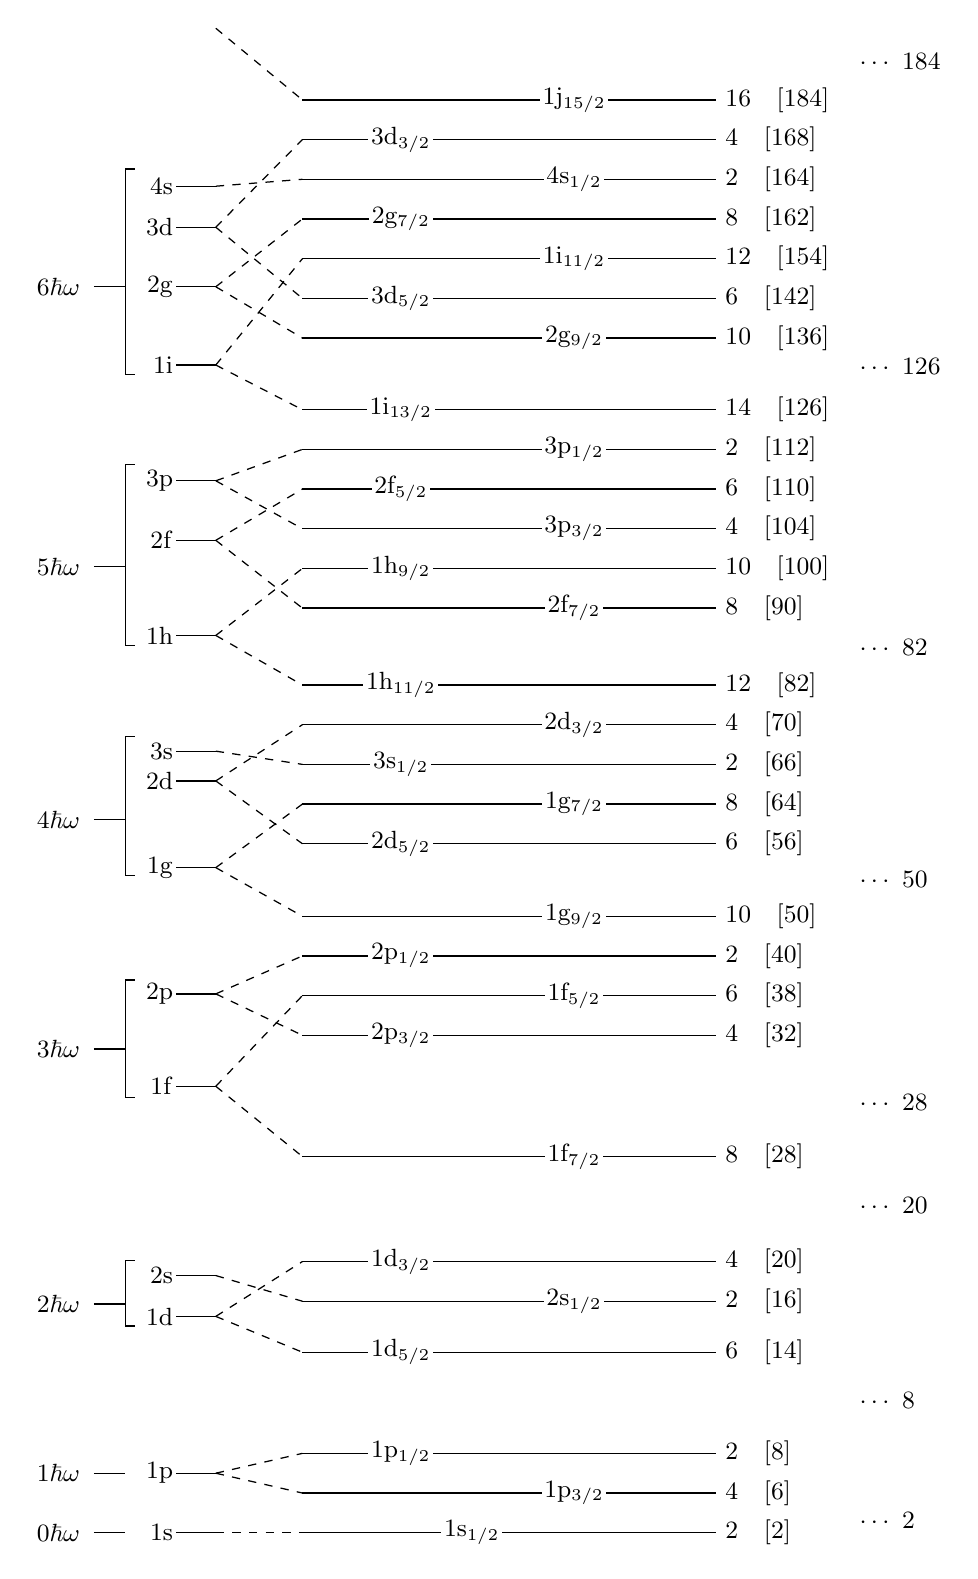
\begin{tikzpicture}[x=1cm,y=.70cm,font=\small,line width=.45pt]
\newcommand{\shelllevel}[4]{%
  \draw (3.25,#1)--(8.5,#1);
  \node[fill=white,inner sep=1pt] at (#2,#1) {$#3$};
  \node[anchor=west,fill=white,inner sep=1pt] at (8.58,#1) {$#4$};}
\newcommand{\leftlevel}[2]{\draw (1.63,#1)--(2.15,#1);\node[anchor=east,fill=white,inner sep=1pt] at (1.65,#1) {$#2$};}
\newcommand{\branch}[2]{\draw[dashed] (2.15,#1)--(3.25,#2);}
% 单粒子能级、简并度及累积核子数（由低到高）。
\shelllevel{0}{5.4}{1\mathrm s_{1/2}}{2\quad[2]}
\shelllevel{0.72}{6.7}{1\mathrm p_{3/2}}{4\quad[6]}
\shelllevel{1.44}{4.5}{1\mathrm p_{1/2}}{2\quad[8]}
\shelllevel{3.275}{4.5}{1\mathrm d_{5/2}}{6\quad[14]}
\shelllevel{4.2}{6.7}{2\mathrm s_{1/2}}{2\quad[16]}
\shelllevel{4.92}{4.5}{1\mathrm d_{3/2}}{4\quad[20]}
\shelllevel{6.825}{6.7}{1\mathrm f_{7/2}}{8\quad[28]}
\shelllevel{9.025}{4.5}{2\mathrm p_{3/2}}{4\quad[32]}
\shelllevel{9.745}{6.7}{1\mathrm f_{5/2}}{6\quad[38]}
\shelllevel{10.465}{4.5}{2\mathrm p_{1/2}}{2\quad[40]}
\shelllevel{11.185}{6.7}{1\mathrm g_{9/2}}{10\quad[50]}
\shelllevel{12.5}{4.5}{2\mathrm d_{5/2}}{6\quad[56]}
\shelllevel{13.22}{6.7}{1\mathrm g_{7/2}}{8\quad[64]}
\shelllevel{13.94}{4.5}{3\mathrm s_{1/2}}{2\quad[66]}
\shelllevel{14.66}{6.7}{2\mathrm d_{3/2}}{4\quad[70]}
\shelllevel{15.38}{4.5}{1\mathrm h_{11/2}}{12\quad[82]}
\shelllevel{16.775}{6.7}{2\mathrm f_{7/2}}{8\quad[90]}
\shelllevel{17.495}{4.5}{1\mathrm h_{9/2}}{10\quad[100]}
\shelllevel{18.215}{6.7}{3\mathrm p_{3/2}}{4\quad[104]}
\shelllevel{18.935}{4.5}{2\mathrm f_{5/2}}{6\quad[110]}
\shelllevel{19.655}{6.7}{3\mathrm p_{1/2}}{2\quad[112]}
\shelllevel{20.375}{4.5}{1\mathrm i_{13/2}}{14\quad[126]}
\shelllevel{21.675}{6.7}{2\mathrm g_{9/2}}{10\quad[136]}
\shelllevel{22.395}{4.5}{3\mathrm d_{5/2}}{6\quad[142]}
\shelllevel{23.115}{6.7}{1\mathrm i_{11/2}}{12\quad[154]}
\shelllevel{23.835}{4.5}{2\mathrm g_{7/2}}{8\quad[162]}
\shelllevel{24.555}{6.7}{4\mathrm s_{1/2}}{2\quad[164]}
\shelllevel{25.275}{4.5}{3\mathrm d_{3/2}}{4\quad[168]}
\shelllevel{25.995}{6.7}{1\mathrm j_{15/2}}{16\quad[184]}
% 未计入自旋--轨道耦合时的轨道组及其分支。
\leftlevel{0}{1\mathrm s}\branch{0}{0}
\leftlevel{1.08}{1\mathrm p}\branch{1.08}{0.72}\branch{1.08}{1.44}
\leftlevel{3.925}{1\mathrm d}\branch{3.925}{3.275}\branch{3.925}{4.92}
\leftlevel{4.6659}{2\mathrm s}\branch{4.6659}{4.2}
\leftlevel{8.1}{1\mathrm f}\branch{8.1}{6.825}\branch{8.1}{9.745}
\leftlevel{9.7763}{2\mathrm p}\branch{9.7763}{9.025}\branch{9.7763}{10.465}
\leftlevel{12.067}{1\mathrm g}\branch{12.067}{11.185}\branch{12.067}{13.22}
\leftlevel{13.64}{2\mathrm d}\branch{13.64}{12.5}\branch{13.64}{14.66}
\leftlevel{14.18}{3\mathrm s}\branch{14.18}{13.94}
\leftlevel{16.2794}{1\mathrm h}\branch{16.2794}{15.38}\branch{16.2794}{17.495}
\leftlevel{18.005}{2\mathrm f}\branch{18.005}{16.775}\branch{18.005}{18.935}
\leftlevel{19.085}{3\mathrm p}\branch{19.085}{18.215}\branch{19.085}{19.655}
\leftlevel{21.1854}{1\mathrm i}\branch{21.1854}{20.375}\branch{21.1854}{23.115}
\leftlevel{22.605}{2\mathrm g}\branch{22.605}{21.675}\branch{22.605}{23.835}
\leftlevel{23.685}{3\mathrm d}\branch{23.685}{22.395}\branch{23.685}{25.275}
\leftlevel{24.4298}{4\mathrm s}\branch{24.4298}{24.555}
\draw[dashed] (2.15,27.295)--(3.25,25.995);
% 谐振子主壳层；括号只标明归组，不表示比例。
\node[anchor=east] at (.55,0) {$0\hbar\omega$};\draw (.6,0)--(1,0);
\node[anchor=east] at (.55,1.08) {$1\hbar\omega$};\draw (.6,1.08)--(1,1.08);
\foreach \low/\high/\mid/\n in {3.75/4.9416/4.15/2,7.9/10.0267/8.775/3,11.9227/14.45/12.9383/4,16.0959/19.385/17.525/5,21.0166/24.7428/22.605/6}{
  \draw (1.12,\low)--(1,\low)--(1,\high)--(1.12,\high);
  \draw (.6,\mid)--(1,\mid);\node[anchor=east] at (.55,\mid) {$\n\hbar\omega$};}
% 壳层闭合数。
\foreach \y/\n in {0.2304/2,2.4023/8,5.9374/20,7.8/28,11.8585/50,16.0591/82,21.1516/126,26.695/184}{
  \node[anchor=west] at (10.2,\y) {$\cdots\ \n$};}
\end{tikzpicture}
}\par
\smallskip{\footnotesize 习题 6.14 图\quad 中子单粒子壳层模型能级示意图}\par
{\footnotesize 右侧分别为能级容纳数及方括号内的累积数；纵向间距不表示能量比例。}
\end{center}}
\answerarea\newpage

\problem{6.15}{\begin{enumerate}
\item 试确定 \nucl{91}{39}{Y} 核的基态和第一激发态的 $I^P$ 值；
\item 估算此原子的处于 $n=1$ 态的电子的能量；
\item 若核的第一激发能为 $555.6\ \mathrm{keV}$，它发出的 $\gamma$ 射线产生的 K 壳层光电子的动能是多少？
\item 随后发出的 K X 射线的能量是多少？
\end{enumerate}}
% layout
\answerarea
\newpage


\chapter{核衰变和核反应}

\problem{7.1}{半衰期为 $30.2\ \mathrm a$ 的 $1\ \mathrm{mg}$ $^{137}\mathrm{Cs}$ 的放射性活度是多少？每秒放出多少 $\beta$ 射线和 $\gamma$ 射线？}
% layout
\answerarea

\problem{7.2}{$1\ \mathrm s$ 内测量到 $^{60}\mathrm{Co}$ 放射源发出的 $\gamma$ 射线有 3700 个，设测量效率为 $10\%$，求它的放射性活度。已知它的半衰期为 $5.27\ \mathrm a$，求它的质量。}
% layout
\answerarea
\newpage

\problem{7.3}{中午 12:00 时试管中 \nucl{25}{11}{Na} 核（$\beta$ 放射性，$T_{1/2}=60\ \mathrm s$）是 $1\ \mu\mathrm g$，求试管内原有的钠原子数到 12:10 还有多少？估算一个钠原子衰变的时间。}
% layout
\answerarea

\problem{7.4}{从 $1.10\ \mathrm{kg}$ 铀矿中含有 $0.20\ \mathrm{kg}$ 铅（$^{206}\mathrm{Pb}$）这一事实估计地球的年龄。已知天然铀含 $99.28\%$ $^{238}\mathrm U$、$0.714\%$ $^{235}\mathrm U$ 和 $0.006\%$ $^{234}\mathrm U$，$^{206}\mathrm{Pb}$ 是 $^{238}\mathrm U$ 衰变系列的稳定产物，$^{238}\mathrm U$ 的半衰期为 $4.5\times10^9\ \mathrm a$，衰变系列中其他核素的半衰期均比它小很多。}
% layout
\answerarea
\newpage

\problem{7.5}{在用 $^{14}\mathrm C$ 测量一具古尸的工作中，已知 $^{14}\mathrm C$ 的 $T_{1/2}=5730\ \mathrm a$，$^{14}\mathrm C$ 的浓度为 $10^{-12}$。
\begin{enumerate}
\item 若取样 $50\ \mathrm g$ 碳测量 $1\ \mathrm h$，得到 $\beta$ 放射性计数为 2500 个，不考虑本底计数，设探测效率为 $90\%$，求它的死亡年代。
\item 若取样 $50\ \mathrm g$ 碳，要求测量精度为 $\pm50\ \mathrm a$，需要多长测量时间？
\item 测量 $1\ \mathrm h$，精度要求同上，问取碳样多少？
\item 设 $N_c$、$N_t$ 和 $N_b$ 分别为真实计数、测量到的总计数和本底计数，即有 $N_c=N_t-N_b$，$N_c$ 的统计误差为
\[
\Delta N_c=\sqrt{(\Delta N_t)^2+(\Delta N_b)^2}=\sqrt{N_t+N_b}.
\]
如果本底计数是 $4000\ \mathrm{h^{-1}}$，测量 $1\ \mathrm h$，精度要求仍同上，要求取碳样多少？
\end{enumerate}}
% layout
\answerarea
\newpage

\problem{7.6}{厚度为 $0.2\ \mathrm{cm}$、面积为 $1\ \mathrm{cm^2}$ 的锡片，放在反应堆热中子道中照射 $1000\ \mathrm h$，以生产放射性核素 \nucl{113}{50}{Sn}。已知 $^{112}_{50}\mathrm{Sn}(\mathrm n,\gamma){}^{113}_{50}\mathrm{Sn}$ 反应截面 $\sigma_\gamma=0.8\ \mathrm b$，$^{112}\mathrm{Sn}$ 核素丰度为 $0.96\%$，锡的密度 $\rho=7.29\times10^3\ \mathrm{kg\,m^{-3}}$，垂直投射的热中子通量为 $5\times10^{16}\ \mathrm{m^{-2}\,s^{-1}}$，$^{113}\mathrm{Sn}$ 的衰变纲图如图所示，\nucl{113}{49}{In} 的 $(1/2)^-$ 能级的内转换系数 $\alpha=0.43$。
\begin{enumerate}
\item 求出堆时 $^{113}\mathrm{Sn}$ 的活度 $A$；
\item 求 5 天以后 $\gamma$ 射线（$393\ \mathrm{keV}$）的强度；
\item 第 5 天从母体 Sn 中分离出子体 $^{113}\mathrm{In}$ 核素，制成 100 份，每份注入一个人体脏器，以诊断疾病，求经一天后体内剩余的 $^{113}\mathrm{In}$ 放射性核素，不考虑人体新陈代谢效应；
\item 求发射的 $\gamma$ 射线的多极性。
\end{enumerate}
\fig{7.6}}
% layout
\answerarea
\newpage

\problem{7.7}{$^{239}\mathrm{Pu}$ 的半衰期可用下法测定：将 $m=120.1\ \mathrm g$ 的 $^{239}\mathrm{Pu}$ 球置于液氦中，液氦体积足以阻止 $\alpha$ 粒子。测得液氦蒸发功率为 $0.231\ \mathrm W$，已知 $E_\alpha=5.144\ \mathrm{MeV}$，求 $^{239}\mathrm{Pu}$ 的半衰期。}
% layout
\answerarea

\problem{7.8}{放射性核素 $^{238}_{94}\mathrm{Pu}$ 已作为宇宙飞行用能源，它是一种半衰期为 $90\ \mathrm a$ 的 $\alpha$ 放射性，问：
\begin{enumerate}
\item 为什么 $^{238}\mathrm{Pu}$ 放射 $\alpha$ 射线而不是氘核？
\item $\alpha$ 射线的能量约为 $5.5\ \mathrm{MeV}$，如有 $238\ \mathrm g$ $^{238}\mathrm{Pu}$，它们释放的功率是多少？
\item 上述能量是仪器运行能量的 8 倍，能用多长时间？
\end{enumerate}}
% layout
\answerarea
\newpage

\problem{7.9}{$^{238}_{94}\mathrm{Pu}$ 主要有三种能量的 $\alpha$ 射线，它们是 $5.499\ \mathrm{MeV}$、$5.457\ \mathrm{MeV}$ 和 $5.358\ \mathrm{MeV}$，分别跃迁到 $^{234}_{92}\mathrm U$ 的基态和第一、第二激发态。求：
\begin{enumerate}
\item $^{234}\mathrm U$ 的第一、第二激发能级的能量；
\item $^{238}\mathrm{Pu}$ 基态和 $^{234}\mathrm U$ 的三个能级的自旋和宇称；
\item 产生的 $\gamma$ 射线能量和多极性。
\end{enumerate}}
% layout
\answerarea

\problem{7.10}{在一个为验证大统一理论的质子衰变实验中，使用了一个含有 $10000\ \mathrm t$ 纯水的水池。
\begin{enumerate}
\item 用切伦科夫辐射探测，设效率为 $100\%$，质子寿命为 $10^{32}\ \mathrm a$，束缚在核内的质子以与自由质子一样的速率衰变，试估计一年内可观测到多少衰变；
\item 设有一种衰变方式为 $\mathrm p\to\pi^0+\mathrm e^+$，$\pi^0\to\gamma+\gamma$，计算光子的最大和最小能量。
\end{enumerate}}
% layout
\answerarea
\newpage

\problem{7.11}{确定核素 \nucl{80}{35}{Br} 是否可能发生 $\beta^-$、$\beta^+$ 衰变和轨道电子俘获，是否可能有 $\alpha$ 衰变和发射中子的衰变，并计算各衰变能。}
% layout
\answerarea

\problem{7.12}{$^{82}\mathrm{Se}$ 可经双 $\beta$ 衰变成 $^{82}\mathrm{Kr}$，已知 $M(^{82}\mathrm{Se})=81.916639\ \mathrm u$、$M(^{82}\mathrm{Kr})=81.91344\ \mathrm u$，求衰变能。}
% layout
\answerarea
\newpage

\problem{7.13}{\begin{enumerate}
\item $^8\mathrm B$ 可经 $\beta^+$ 衰变到 $^8\mathrm{Be}$，如图所示。这是太阳产生中微子的一个来源，简要说明哪些种 $\beta^+$ 衰变构成中微子谱的主要来源。
\item 除上述外，太阳还通过 $\mathrm p+\mathrm p\to\mathrm d+\beta^++\nu_e$ 聚变反应产生中微子，试问这些中微子作用在 $^1\mathrm H$ 靶和 $^2\mathrm H$ 靶上能否产生反应？能产生什么反应？已知下列原子的质量剩余（以 MeV 作单位）为
\[
\begin{array}{ccccc}
{}^1\mathrm H&\mathrm n&{}^2\mathrm H&{}^8\mathrm B&{}^8\mathrm{Be}\\
7.289&8.071&13.136&22.922&4.942
\end{array}
\]
\end{enumerate}
\fig{7.13}}
% layout
\answerarea
\newpage

\problem{7.14}{原子核 $^{69}\mathrm{Zn}$ 处于能量为 $436\ \mathrm{keV}$ 的同质异能态时，试求它发射 $\gamma$ 光子后的反冲动能和发射内转换电子后的反冲动能；若 $^{69}\mathrm{Zn}$ 处于高激发态，可以发射中子，试求发射 $436\ \mathrm{keV}$ 中子后的反冲能。}
% layout
\answerarea

\problem{7.15}{$^{182}_{73}\mathrm{Ta}$ 的激发态能量为 $137\ \mathrm{keV}$，寿命为 $2\times10^{-15}\ \mathrm s$，用同样能量的 $\gamma$ 射线入射到 $^{182}\mathrm{Ta}$ 核时，能否使核共振激发？}
% layout
\answerarea
\newpage

\problem{7.16}{反应 $^{10}\mathrm B+\mathrm d\to{}^8\mathrm{Be}+\alpha+17.85\ \mathrm{MeV}$，当 d 束能量为 $0.6\ \mathrm{MeV}$ 时，在 $90^\circ$ 方向观测到四种能量的 $\alpha$ 射线，它们是 $12.2$、$10.2$、$9.0$ 和 $7.5\ \mathrm{MeV}$，求 $^8\mathrm{Be}$ 的激发能。}
% layout
\answerarea

\problem{7.17}{氘核吸收 $6\ \mathrm{MeV}$ $\gamma$ 射线后发生分解，如果在与入射光子成 $90^\circ$ 角方向上探测到质子，求反应 $Q$ 值和氘核结合能、中子和质子的动能以及中子的飞出方向。}
% layout
\answerarea
\newpage

\problem{7.18}{已观测到下列两核反应：
\[
{}^{14}\mathrm N+\alpha={} ^{17}\mathrm O+\mathrm p-1.26\ \mathrm{MeV},
\]
\[
{}^{16}\mathrm O+\mathrm d={} ^{14}\mathrm N+\alpha+3.13\ \mathrm{MeV}.
\]
如用 d 打 $^{16}\mathrm O$ 时也形成 $^{17}\mathrm O+\mathrm p$，计算 d 能量为 $1.00\ \mathrm{MeV}$ 时在实验室系 $0^\circ$ 和 $90^\circ$ 方向射出的质子的动能。}
% layout
\answerarea

\problem{7.19}{在什么条件下反应 $^7\mathrm{Li}(\mathrm p,\mathrm n){}^7\mathrm{Be}$ 能实现？在这个阈值下的中子实验室能量是多少？}
% layout
\answerarea
\newpage

\problem{7.20}{探测器面积为 $2\ \mathrm{cm^2}$，覆盖一层自发裂变重核，平均寿命为 $\frac13\times10^9\ \mathrm a$，每秒观测到 20 个裂变事例。若放到通量为 $10^{11}\ \mathrm{cm^{-2}\,s^{-1}}$ 的均匀中子流中，探测到的裂变数为 $120\ \mathrm{s^{-1}}$，试问中子诱发裂变截面为多大？}
% layout
\answerarea

\newpage

\problem{7.21}{1987 年 3 月在两个地下大中微子探测器中同时记录到一个由若干中微子事例组成的爆发，它们出现在几秒钟的隔内，这是由于一个靠近银河系边缘的超新星 1987A 的突然爆发所发出的 $10\ \mathrm{MeV}$ 能区的 $\nu$ 和 $\bar\nu$ 引起的。各个中微子探测器是由一个在约 $1000\ \mathrm m$ 深的矿井中的盛有约 $5000\ \mathrm t$ 纯水的容器组成的，水用一大组光电倍增管围绕，以探测相对论带电粒子产生的切伦科夫辐射。$10\ \mathrm{MeV}$ 能区的中微子与纯水主要作用是
\[
\text{（a）}\ \nu+\mathrm e\to\nu+\mathrm e,\qquad
\text{（b）}\ \bar\nu+\mathrm p\to\mathrm n+\mathrm e^+.
\]
\begin{enumerate}
\item $10\ \mathrm{MeV}$ 的中微子在（a）作用中产生的出射电子最大能量是多少？
\item 两反应中的出射带电粒子在质心系中有各向同性分布，哪种反应的出射电子在实验室系中角分布将指示入射中微子方向？
\item 两探测器的事例爆发被推断为 $\nu$（实际是 $\bar\nu$），它们的能量为 $10\!\sim40\ \mathrm{MeV}$。设所有这些中微子是同一时刻从那个超新星爆发中发射的，在到达地球时通过约 $170000$ 光年的距离，它们到达时间有 $2\ \mathrm s$ 弥散，试估计中微子质量上限。
\end{enumerate}}
% layout
\answerarea
\newpage


\chapter{射线与物质的相互作用}

\problem{8.1}{$^{137}\mathrm{Cs}$ 放射源发出的 $\gamma$ 射线能量是 $662\ \mathrm{keV}$，当它通过高纯锗半导体探测器时，试计算：
\begin{enumerate}
\item 光电子的能量；
\item 康普顿散射光子和反冲电子的最大和最小能量；
\item 连续两次 $90^\circ$ 康普顿散射光子的能量；
\item 激活的 K X 射线的能量。
\end{enumerate}}
% layout
\answerarea

\problem{8.2}{在一个用 X 射线激发的 X 荧光分析测量中，X 射线源为同位素 $^{238}\mathrm{Pu}$，放出的主要两条 X 射线的能量是 $17.3\ \mathrm{keV}$ 和 $13.6\ \mathrm{keV}$，用 Si(Li) 探测器测量样品发出的 X 射线。探测器和源相对样品来说放在同一边，可以近似地认为产生的 X 射线方向与源发出的 X 射线方向相反，Si(Li) 不能直接测到源发出的 X 射线。测量结果表明除了有样品的特征 X 射线外，还有 4 个峰，它们是怎样产生的？计算它们的能量。}
% layout
\answerarea
\newpage

\problem{8.3}{试求波长为 $337.1\ \mathrm{nm}$ 的氮分子激光束与静止电子以及和 $100\ \mathrm{keV}$ 能量的电子对头撞后的反散射光子的能量。}
% layout
\answerarea

\problem{8.4}{慢中子束通过一块镉板后强度减弱到原来的 $5\%$，镉的 $A=112$，$\rho=8.7\times10^3\ \mathrm{kg\,m^{-3}}$，中子是一个一个地被吸收，镉的吸收截面为 $2500\ \mathrm b$，求所需镉的厚度。}
% layout
\answerarea
\newpage

\problem{8.5}{已知铜和锌的 $\mathrm K_\alpha$ X 射线的波长分别为 $0.1539\ \mathrm{nm}$ 和 $0.1434\ \mathrm{nm}$，镍的 K 吸收限为 $0.1489\ \mathrm{nm}$，它对铜和锌的 $\mathrm K_\alpha$ 射线的质量吸收系数分别为 $0.480$ 和 $32.5\ \mathrm{m^2\,kg^{-1}}$，试问：
\begin{enumerate}
\item 为使黄铜的这两条 $\mathrm K_\alpha$ X 射线的相对强度之比提高 10 倍，需用多厚的镍吸收片？
\item 通过此吸收片后两条射线各减弱到多少？（已知镍的密度为 $9.04\times10^3\ \mathrm{kg\,m^{-3}}$。）
\end{enumerate}}
% layout
\answerarea

\problem{8.6}{在使用 X 光机和 $\gamma$ 放射源时，常需用铅板来屏蔽，以达到防护的目的，求为使 $^{137}\mathrm{Cs}$ 源的 $\gamma$ 射线（$662\ \mathrm{keV}$）和 $50\ \mathrm{keV}$ X 光机的 X 射线减弱到 $1/1000$ 所需的铅厚。（已知它们的质量吸收系数分别为 $0.010\ \mathrm{m^2\,kg^{-1}}$ 和 $0.849\ \mathrm{m^2\,kg^{-1}}$。）}
% layout
\answerarea
\newpage

\problem{8.7}{试证明正负电子对不能被单个孤立光子产生，只能发生在粒子附近。求光子在原子核或核外电子附近产生电子对效应的阈能。}
% layout
\answerarea

\problem{8.8}{泡室是一种径迹探测器，能把带电粒子的径迹拍成照片。一个光子通过泡室时产生了一个电子--正电子对，泡室放在强度 $B=0.20\ \mathrm T$ 的均匀磁场中，从照片中发现它们具有相反的曲率半径 $r=2.5\times10^{-2}\ \mathrm m$，求此光子的能量。}
% layout
\answerarea
\newpage

\problem{8.9}{在一束能量为 $10.0\ \mathrm{eV}$ 的电子射入单原子气体后，气体发生下列波长的光：$140.2\ \mathrm{nm}$、$253.6\ \mathrm{nm}$ 和 $313.2\ \mathrm{nm}$，波长为 $253.6\ \mathrm{nm}$ 的光强显著地大于另外两个波长的光强，试问出射电子具有多大能量？}
% layout
\answerarea

\problem{8.10}{试求为进行锌的 K X 荧光分析所需要的最小 X 射线、电子和质子的能量。}
% layout
\answerarea
\newpage

\problem{8.11}{试求能量为 $5.3\ \mathrm{MeV}$ 的 $\alpha$ 粒子
\begin{enumerate}
\item 穿过铝和铅的电离损失之比；
\item 穿过铝的电离损失值；
\item 和同样能量的氘核穿过铝的电离损失之比。
\end{enumerate}}
% layout
\answerarea

\problem{8.12}{在一个充 $1\ \mathrm{atm}$ 空气的云室内，$5.3\ \mathrm{MeV}$ 的 $\alpha$ 粒子显示出 $4\ \mathrm{cm}$ 长的径迹，问大约要观测多少个径迹才可能有一次机会发现由于核碰撞引起的大角弯折？}
% layout
\answerarea
\newpage

\problem{8.13}{求在液氮温度下处于三个最低转动态的 HD 分子的相对数。}
% layout
\answerarea

\problem{8.14}{求温度为 $3000\ \mathrm K$ 时处在基态、第一激发态和第二激发态的氢原子数目之比。}
% layout
\answerarea
\newpage

\problem{8.15}{原子在寿命为 $1.5\times10^{-8}\ \mathrm s$ 和 $2\times10^{-8}\ \mathrm s$ 的两激发态之间跃迁，产生相应于波长为 $532.0\ \mathrm{nm}$ 的谱线，试确定谱线的自然宽度。}
% layout
\answerarea

\problem{8.16}{在加热温度为 $440\ {}^\circ\mathrm C$ 时钠蒸气压为 $1\ \mathrm{mmHg}$。
\begin{enumerate}
\item 求此条件下钠蒸气原子共振谱线的自然宽度、碰撞展宽和多普勒展宽（已知钠的 $3\mathrm P$ 能级寿命为 $16\ \mathrm{ns}$）；
\item 能否观测到从 $4\mathrm D\to3\mathrm P$ 的 $568.822\ \mathrm{nm}$ 的发射和吸收谱线？
\end{enumerate}}
% layout
\answerarea
\newpage

\problem{8.17}{氢的 $2\mathrm P$ 能级的电偶极辐射的自发辐射寿命是 $1.596\ \mathrm{ns}$，试估计单电离氦和双电离锂的 $2\mathrm P$ 能级寿命。}
% layout
\answerarea

\newpage


\chapter{粒子物理}

\problem{9.1}{试说明由于违反什么守恒律，使下列反应不能发生：
\begin{enumerate}
\item $\mathrm n\to\mathrm p+\mathrm e^-$；
\item $\mathrm n\to\pi^++\mathrm e^-+\nu_e$；
\item $\mathrm n\to\mathrm p+\pi^-$；
\item $\mathrm n\to\mathrm p+\gamma$。
\end{enumerate}}
% layout
\answerarea

\problem{9.2}{试计算当 $\gamma$ 射线和静止电子相互作用而产生正、负电子对的阈能。}
% layout
\answerarea
\newpage

\problem{9.3}{判断下列各反应中哪些是禁戒的，若是允许的反应，请说明是属于哪种相互作用。
\begin{enumerate}
\item $\mathrm p\to\pi^++\mathrm e^++\mathrm e^-$；
\item $\Lambda^0\to\mathrm p+\pi^-$；
\item $\mu^-\to\mathrm e^-+\bar\nu_e+\nu_\mu$；
\item $\mathrm n+\mathrm p\to\Sigma^++\Lambda^0$；
\item $\Sigma^+\to\mathrm p+\gamma$。
\end{enumerate}}
% layout
\answerarea

\problem{9.4}{讨论 $\Omega$ 超子可能的衰变方式，并说明为什么它只能通过弱作用衰变。}
% layout
\answerarea
\newpage

\problem{9.5}{用高能质子轰击液氢靶时，求产生 $\pi$ 介子的阈能。（氘核的质量为 $1875.6\ \mathrm{MeV}$。）}
% layout
\answerarea

\problem{9.6}{若规定 $\mathrm K^+$ 介子的奇异数为 $+1$，试定出 $\mathrm K^-$ 和 $\Sigma^+$ 粒子的奇异数。}
% layout
\answerarea
\newpage

\problem{9.7}{已知带电 $\pi$ 介子的寿命为 $2.6\times10^{-8}\ \mathrm s$，在实验室中测得飞行中 $\pi$ 介子的寿命为 $75\ \mathrm{ns}$，求 $\pi$ 介子的速度、总能量、动能和动量。}
% layout
\answerarea

\problem{9.8}{求静止 $\pi$ 介子衰变产生的 $\mu$ 子和中微子的动能。}
% layout
\answerarea
\newpage

\problem{9.9}{设一个介子衰变成两个自旋为零的中性 $\pi$ 介子，这个介子的自旋可能取哪些值？}
% layout
\answerarea

\problem{9.10}{一个高速电子与静止电子碰撞，求反应产生正电子的阈动量。}
% layout
\answerarea
\newpage

\problem{9.11}{用 $\pi^+$ 介子轰击静止质子时，测到有质量为 $1690\ \mathrm{MeV}$ 的共振态，求入射 $\pi^+$ 介子的最低动能。}
% layout
\answerarea

\problem{9.12}{$\pi^-$ 介子（$J^P=0^-$）和氘核（$J^P=1^+$）组成原子基态。$\pi^-$ 最终被氘核俘获，并发生反应 $\pi^-+\mathrm d\to\mathrm n+\mathrm n$，求：
\begin{enumerate}
\item 产生的中子对的轨道角动量；
\item 中子系统的总自旋角动量。
\end{enumerate}}
% layout
\answerarea
\newpage

\problem{9.13}{实验中观察到下列过程：$\Xi^-\to\Lambda^0+\pi^-$，试分析其同位旋、奇异数守恒情况，并说明这一过程是属哪种相互作用过程。}
% layout
\answerarea

\problem{9.14}{请写出强子 $\overline{\mathrm K}(\mathrm s\bar{\mathrm d})$、$\varphi(\mathrm s\bar{\mathrm s})$、$\Delta(\mathrm u\mathrm u\mathrm u)$、$\Xi(\mathrm s\mathrm s\mathrm d)$、$\overline\Omega(\bar{\mathrm s}\bar{\mathrm s}\bar{\mathrm s})$ 的电荷 $Q$、同位旋 $I$ 及 $I_3$、奇异数 $S$ 和重子数 $B$。}
% layout
\answerarea
\newpage

\problem{9.15}{阐述电子偶素 $^3\mathrm S_1$ 状态不可能衰变为两个光子的理由。}
% layout
\answerarea

\problem{9.16}{试证明由粲夸克和反粲夸克 $c\bar c$ 组成的介子不可能具有 $J^{PC}=1^{-+}$ 的状态。}
% layout
\answerarea
\newpage

\problem{9.17}{在光子、中微子、中子和电子中，试问：
\begin{enumerate}
\item 哪些不参与电磁相互作用？
\item 哪些不参与强相互作用？
\item 哪些不参与弱相互作用？
\end{enumerate}}
% layout
\answerarea

\problem{9.18}{在北京正负电子对撞机上的实验中，利用反应 $\mathrm e^++\mathrm e^-\to\mathrm J/\psi$，测到质量为 $3.1\ \mathrm{GeV}$ 的 $\mathrm J/\psi$ 粒子，求这一反应的阈能。如果以 $\mathrm e^+$ 撞击静止的 $\mathrm e^-$，则产生 $\mathrm J/\psi$ 的阈能为多大？}
% layout
\answerarea
\newpage

\problem{9.19}{$\mathrm J/\psi$ 粒子是由粲夸克和反粲夸克组成的，已知它的 $J^{PC}=1^{--}$，请给出这个粲夸克素的轨道角动量、自旋角动量、同位旋量子数。}
% layout
\answerarea

\problem{9.20}{已知 $\Xi^-$ 的 $Q=-1$，$B=1$，$S=-2$。请写出它的夸克组成，以及它的同位旋多重态中其他粒子的 $Q$、$B$ 和 $S$。}
% layout
\answerarea
\newpage

\problem{9.21}{$\rho^-$ 介子是由 $\pi^-$ 和 p 散射得到的介子共振态，其反应为 $\pi^-+\mathrm p\to\rho^-+\mathrm p$，试由守恒关系给出 $\rho^-$ 介子的同位旋、同位旋第三分量、奇异数和重子数。}
% layout
\answerarea

\problem{9.22}{实验测得 $\rho$ 介子的质量宽度为 $150\ \mathrm{MeV}$，求它的平均寿命。}
% layout
\answerarea
\newpage

\problem{9.23}{指出并说明下列哪些反应或衰变是守恒定律允许的：
\begin{enumerate}
\item $\mathrm p\to\pi^++\pi^0$；
\item $\pi^-+\mathrm p\to\mathrm K^++\Sigma^-$；
\item $\pi^-\to\mathrm e^-+\gamma$；
\item $\mathrm p\to\Sigma^++\pi^0$；
\item $\mathrm p+\mathrm p\to\mathrm n+\mathrm p+\pi^++\pi^-+\pi^0$。
\end{enumerate}}
% layout
\answerarea
\newpage

\problem{9.24}{衰变过程 $\Lambda\to\mathrm p+\pi^-$ 是一个弱作用过程，请给出判断的理由。}
% layout
\answerarea

\newpage

\problem{9.25}{试判断下列衰变过程哪些是可能发生的，哪些是不可能发生的，并加以说明。
\begin{enumerate}
\item $\pi^+\to\mu^++\nu_\mu$；
\item $\pi^-\to\pi^++\mathrm e^-+\mathrm e^-$；
\item $\pi^0\to\mathrm e^-+\mathrm p$；
\item $\mathrm p\to\mathrm n+\mathrm e^++\nu_e$；
\item $\mathrm n\to\mathrm p+\mathrm e^-+\bar\nu_e$。
\end{enumerate}}
% layout
\answerarea
\newpage

\problem{9.26}{根据夸克模型，说明强子中含有的价夸克或反夸克数。}
% layout
\answerarea

\newpage

\problem{9.27}{指出下列过程产生的 $\nu$ 中哪些是中微子，哪些是反中微子，并写出是属于哪种类型的：
\begin{enumerate}
\item $\Lambda^0\to\mathrm p+\mu^-+\nu$；
\item $\Sigma^+\to\mu^++\nu+\mathrm n$；
\item $\tau^+\to\mathrm e^++\nu+\nu$；
\item $\mu^-\to\mathrm e^-+\nu+\nu$；
\item $\mathrm K^+\to\mu^++\nu$。
\end{enumerate}}
% layout
\answerarea
\newpage

\problem{9.28}{假设某种玻色子的下列量子数都不为 0，试问这种玻色子和它的反粒子的哪一个量子数是相同的？
\begin{enumerate}
\item 奇异数；
\item 粲数；
\item 内禀宇称；
\item 磁矩；
\item 电荷。
\end{enumerate}}
% layout
\answerarea

\problem{9.29}{$\mathrm K^+$ 介子可以衰变为三个 $\pi$ 介子，$\mathrm K^+\to\pi^++\pi^-+\pi^+$，试计算 $\pi$ 介子的最大能量和平均能量。}
% layout
\answerarea
\newpage

\problem{9.30}{下列四组粒子中，哪一组是属于完备的同位旋多重态？
\begin{enumerate}
\item $(\rho^+,\rho^-)$；
\item $(\mathrm K^+,\mathrm K^-)$；
\item $(\mathrm K^0,\overline{\mathrm K}{}^0)$；
\item $(\Sigma^+,\Sigma^0,\Sigma^-)$。
\end{enumerate}}
% layout
\answerarea

\newpage

\problem{9.31}{费米子和反费米子系统的空间宇称 $\eta_P$ 与电荷宇称 $\eta_C$ 由系统的相对运动轨道角动量 $L$ 和总自旋 $S$ 决定，下列表达式中哪个是正确的？
\begin{enumerate}
\item $\eta_P=(-1)^L$，$\eta_C=(-1)^{L+S}$；
\item $\eta_P=(-1)^{L+1}$，$\eta_C=(-1)^{S+1}$；
\item $\eta_P=(-1)^{L+S}$，$\eta_C=(-1)^{L+1}$；
\item $\eta_P=(-1)^{L+1}$，$\eta_C=(-1)^{L+S}$。
\end{enumerate}}
% layout
\answerarea
\newpage

\problem{9.32}{已知共振态 $\psi(3686)$ 的夸克组成为 $2^3\mathrm S_1\ (c\bar c)$，其衰变总宽度 $\Gamma=277\ \mathrm{keV}$，衰变到正负电子对的分宽度 $\Gamma_{ee}=2.14\ \mathrm{keV}$。
\begin{enumerate}
\item 画出衰变末态为正负电子不变质量谱的形状（注意横坐标的比例），在不变质量谱上标出 $\psi(3686)$ 的质量、不变质量谱的半高全宽（FWHM）应该取何值（假定谱仪的质量分辨小于 $1\ \mathrm{keV}$）？
\item 计算该共振态的平均寿命。
\item 写出 $\psi(3686)$ 的 $I^G(J^{PC})$。
\end{enumerate}}
% layout
\answerarea
\newpage

\problem{9.33}{设能量在 GeV 的中微子的反应截面约为 $10^{-38}\ \mathrm{cm^2}$，试估算中微子在铀中的平均自由程。}
% layout
\answerarea

\problem{9.34}{由粒子表得到 $\Sigma$ 粒子的质量分别为 $1189.4\ \mathrm{MeV}$（$\Sigma^+$）、$1192.6\ \mathrm{MeV}$（$\Sigma^0$）和 $1197.4\ \mathrm{MeV}$（$\Sigma^-$），试由它们的夸克组成来估算 d 夸克和 u 夸克的质量差。}
% layout
\answerarea
\newpage


\end{document}
